\documentclass[../TDE1-E2.tex]{subfiles}%

\begin{document}
\section[s]"1"{Conventions et puissances}

\enonce{%
  \begin{minipage}{0.30\linewidth}
  Pour le circuit ci-contre :
\end{minipage}
\begin{minipage}{0.70\linewidth}
  \begin{center}
    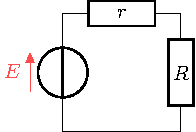
\includegraphics[width=.3\linewidth]{convs_plain}
  \end{center}
\end{minipage}
}%

\QR{%
  \begin{enumerate}[label=\alph* --, leftmargin=20pt]
          \item Flécher les courants et les tensions en convention récepteur
                pour chaque dipôle.
          \item Exprimer la puissance (notée $\Pc(R)$ pour le dipôle $R$)
            associée à chaque dipôle.
          \item En faisant un bilan de puissance reçue par le système,
                déterminer l'expression du courant I.
        \end{enumerate}
}{%
  \vspace{-15pt}
\begin{tcbraster}[raster columns=7, raster equal height=rows]
    \begin{tcn}[raster multicolumn=2](data){Schéma}
        \begin{center}
            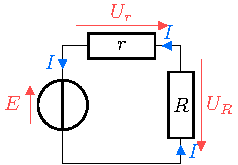
\includegraphics{convs_a}
        \end{center}
    \end{tcn}
    \begin{tcn}[raster multicolumn=2](tool)""{Calcul}
        \begin{itemize}[leftmargin=20pt]
            \item $\Pc_{\text{r}}(E) = -EI$
            \item $\Pc_{\text{r}}(r) = rI^2$
            \item $\Pc_{\text{r}}(R) = RI^2$
        \end{itemize}
    \end{tcn}
    \begin{tcn}[raster multicolumn=3](appl)'r'{Application}
        On a $\sum \Pc_{\text{f}} = \sum \Pc_{\text{r}}$, donc d'après
        la question précédente~:
        \begin{align*}
            0         & = -EI + rI^2 + RI^2\\
            I(r+R)    & = E\\
            \Aboxed{I & = \frac{E}{r+R}}
        \end{align*}
    \end{tcn}
\end{tcbraster}
}%

\QR{%
        \begin{enumerate}[label=\alph* --, leftmargin=20pt]
          \item Reproduire le circuit et flécher les courants et tensions en
                convention générateur pour chaque dipôle.
          \item Exprimer la puissance associée à chaque dipôle.
          \item En faisant un bilan de puissance, déterminer l'expression du
                courant I.
        \end{enumerate}
}{%
  \vspace{-15pt}
\begin{tcbraster}[raster columns=7, raster equal height=rows]
    \begin{tcn}[raster multicolumn=2](data){Schéma}
        \begin{center}
            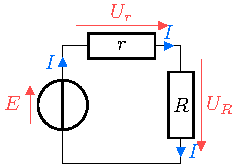
\includegraphics{convs_b}
        \end{center}
    \end{tcn}
    \begin{tcn}[raster multicolumn=2](tool)""{Calcul}
        \begin{itemize}[leftmargin=20pt]
            \item $\Pc_{\text{f}}(E) = EI$
            \item $\Pc_{\text{f}}(r) = -rI^2$
            \item $\Pc_{\text{f}}(R) = -RI^2$
        \end{itemize}
    \end{tcn}
    \begin{tcn}[raster multicolumn=3](appl)'r'{Application}
        On a $\sum \Pc_{\text{f}} = \sum \Pc_{\text{r}}$, donc d'après
        la question précédente~:
        \begin{align*}
            EI - rI^2 - RI^2 & = 0\\
            I(r+R)           & = E\\
            \Aboxed{I        & = \frac{E}{r+R}}
        \end{align*}
    \end{tcn}
\end{tcbraster}
}%

\QR{%
        \begin{enumerate}[label=\alph* --, leftmargin=20pt]
          \item Reproduire le schéma et flécher les courants et tensions de
                chaque dipôle en fonction de sa nature (récepteur / générateur).
          \item Exprimer la puissance associée à chaque dipôle.
          \item En faisant un bilan de puissance reçu par le système,
                déterminer l'expression du courant I.
        \end{enumerate}
}{%
  \vspace{-15pt}
\begin{tcbraster}[raster columns=7, raster equal height=rows]
    \begin{tcn}[raster multicolumn=2](data){Schéma}
        \begin{center}
            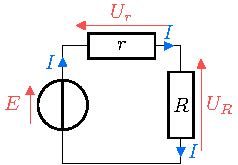
\includegraphics{convs_c}
        \end{center}
    \end{tcn}
    \begin{tcn}[raster multicolumn=2](tool)""{Calcul}
        \begin{itemize}[leftmargin=20pt]
            \item $\Pc_{\text{f}}(E) = EI$
            \item $\Pc_{\text{r}}(r) = rI^2$
            \item $\Pc_{\text{r}}(R) = RI^2$
        \end{itemize}
    \end{tcn}
    \begin{tcn}[raster multicolumn=3](appl)'r'{Application}
        On a $\sum \Pc_{\text{f}} = \sum \Pc_{\text{r}}$~: avec les
        conventions adaptées, on a~:
        \begin{align*}
            EI        & = rI^2 + RI^2\\
            I(r+R)    & = E\\
            \Aboxed{I & = \frac{E}{r+R}}
        \end{align*}
    \end{tcn}
\end{tcbraster}
}%

\QR{%
  Comparer les résultats obtenus aux réponses précédentes.
}{%
  ~
  \vspace{-15pt}
    \begin{tcn}[width=\linewidth](impo){Conclusion}
        On trouve bien toujours la même valeur de l'intensité dans le circuit,
        ce qui montre bien que les conventions ne sont que des conventions et ne
        changent pas la manière dont la physique fonctionne ensuite. Il faut
        noter cependant que le $I$ du premier schéma n'est pas le $I$ des
        schémas 2 et 3, étant donné que le sens n'est pas le même~: les
        intensitées sont opposées.
    \end{tcn}
}%

\end{document}
